

\chapter{Chosen Ciphertext Secure Public Key Encryption}

    \section{Chosen Ciphertext Security}
        \begin{itemize}
            \item As in the case of private key encryption, we also want to consider active adversaries against public key encryption
            \item Chosen ciphertext attacks are a bigger concern in public key encryption as receivers expect encrypted messages from unknown senders
            \item Consider scenario where server signals if ciphertext is valid or invalid
        \end{itemize}
        \begin{center}
	        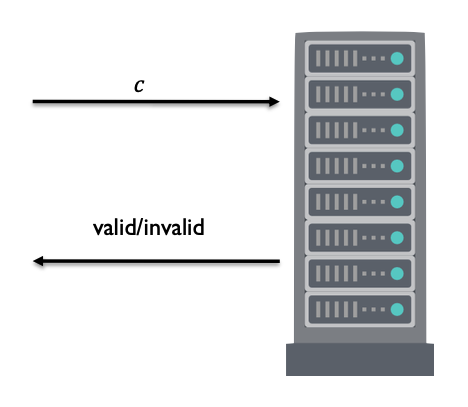
\includegraphics[width=80mm]{Graphics/Chosen Ciphertext Secure Public Key Encryption/cca1.png}
        \end{center}

    \section{RSA PKCS $\#$1}
        \begin{center}
	        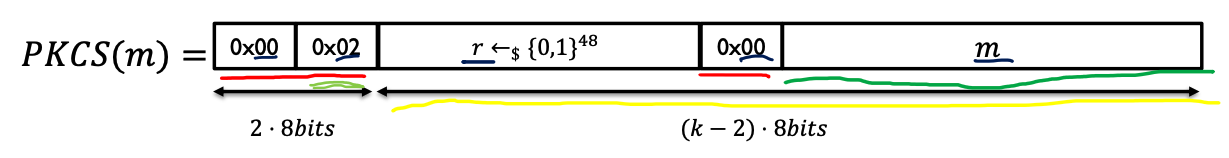
\includegraphics[width=140mm]{Graphics/Chosen Ciphertext Secure Public Key Encryption/cca2.png}
        \end{center}
        \begin{itemize}
            \item $KeyGen$ as in textbook RSA $(N,e,d)$
            \item $Enc(pk,m)$: Compute an output $c \leftarrow (PKCS(m))^e\ mod\ N$
            \item $Dec(sk,c)$: Compute $m' \leftarrow c^d$, if $m'$ is a correct PKCS encoding output decoded value $m$ (lower order bits of $m'$, otherwise output 'invalid')\\
            \item Observation: $m' \in \{0,...,N-1\}$ is correct encoding if and only if $2B \leq m' \leq 3B-1$, where $B = 2^{(k-2)8}$
        \end{itemize}
    
    \section{Bleichenbacher's Attack}
        \begin{itemize}
            \item It turns out, for RSA PKCS$\#$1 a server which signals if a ciphertext is valid can be abused to implement a decryption oracle!
            \item Idea of the Attack:
        \end{itemize}
        \begin{center}
	        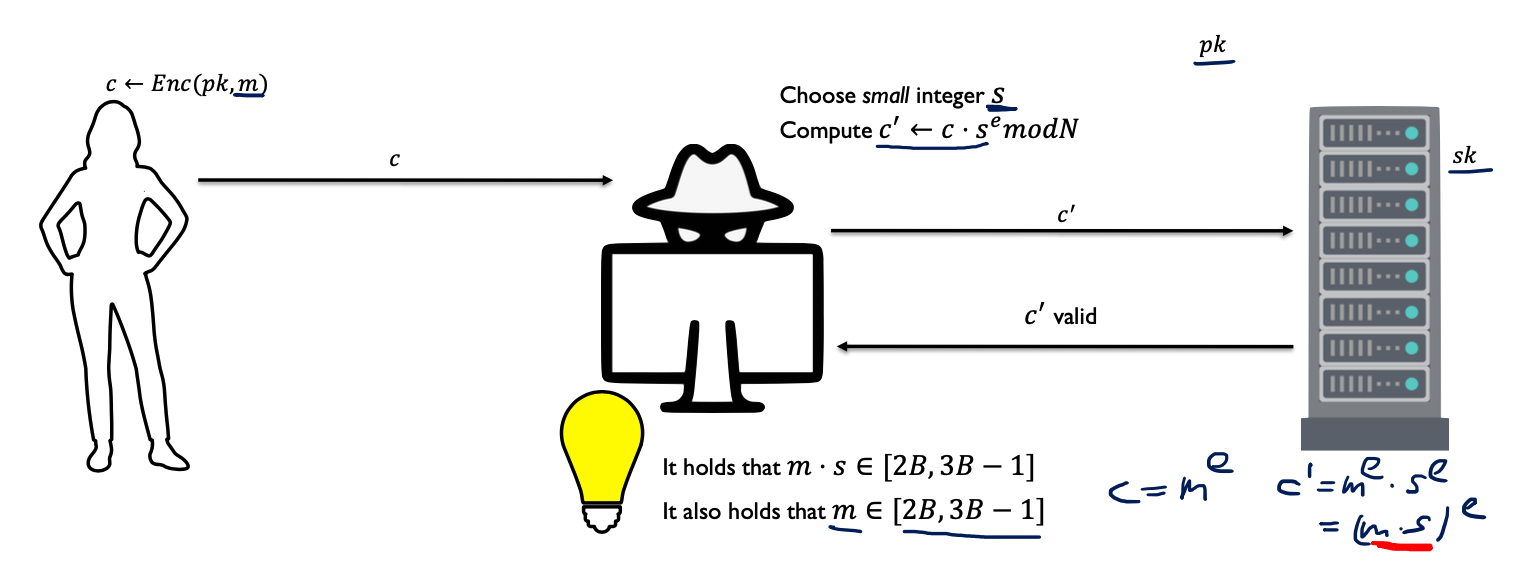
\includegraphics[width=160mm]{Graphics/Chosen Ciphertext Secure Public Key Encryption/cca3.png}
        \end{center}
        \begin{center}
	        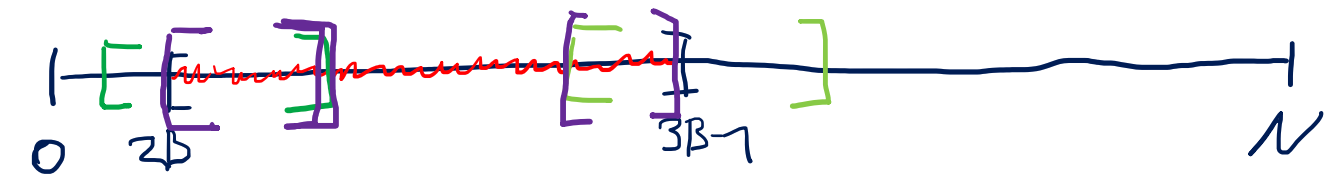
\includegraphics[width=160mm]{Graphics/Chosen Ciphertext Secure Public Key Encryption/cca4.png}
        \end{center}
        Let $m \in [2B,3B-1]$, $m \cdot s \in [2B,3B-1]$ and $F: m \mapsto m \cdot s$ with $F^{-1}([2B,3B-1])$:
        $$m \cdot s \ mod\ N \in [2B,3B-1] \Rightarrow \exists r \in \mathbb{Z}_{\geq 0} s\cdot m - r \cdot N \in [2B,3B-1]$$
        $$\Leftrightarrow \exists r \geq 0 \ \text{s.t.}\  M \in [\frac{2B + r \cdot N}{S},\frac{3B-1 + r \cdot N}{S}] \  \text{given}\  s \geq \frac{N}{3B}$$

\newpage
    \section{Chosen Ciphertext Security of Public Key Encryption}
        \begin{definition}[$IND-CCA$-\textbf{secure} encryption scheme's]
            An encryption scheme $(KeyGen,Enc,Dec)$ is $IND-CCA$-\textbf{secure}, if it holds for \textbf{every PPT-adversary} $\mathcal{A}$ there exists a negligible function $v$ s.t. for all $\lambda \in \mathcal{N}$
            $$Pr[IND-CCA_{\mathcal{A}}(\lambda)=1] < \frac{1}{2} + v(\lambda)$$
        \end{definition}
        \begin{center}
	        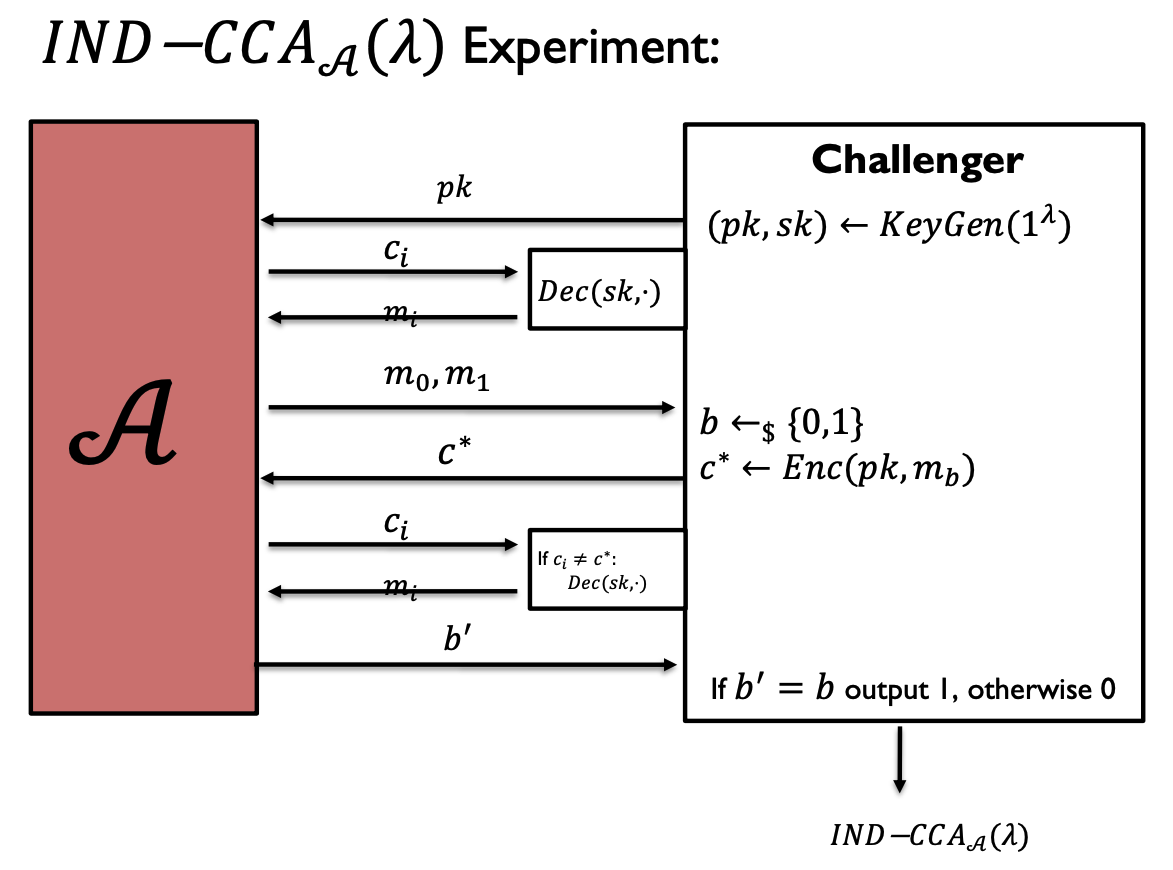
\includegraphics[width=180mm]{Graphics/Chosen Ciphertext Secure Public Key Encryption/cca5.png}
        \end{center}

\newpage
    \section{Chosen Ciphertext Security of Key Encapsulation Mechanisms}
        \begin{definition}[$IND-CCA$-\textbf{secure} KEM's]
            A KEM $(KeyGen,Encaps,Decaps)$ is $IND-CCA$-\textbf{secure}, if it holds for \textbf{every PPT-adversary} $\mathcal{A}$ there exists a negligible function $v$ s.t. for all $\lambda \in \mathcal{N}$
            $$Pr[IND-CCA_{\mathcal{A}}(\lambda)=1] < \frac{1}{2} + v(\lambda)$$
        \end{definition}
        \begin{center}
	        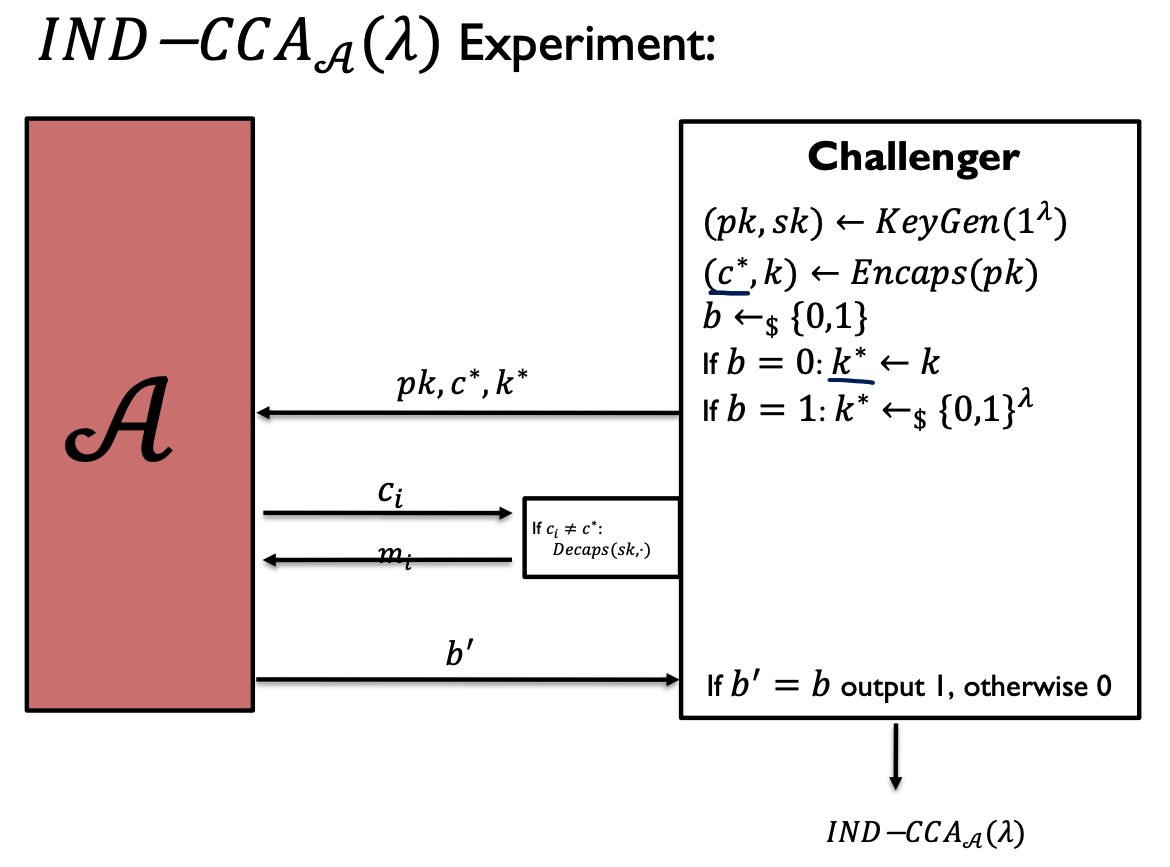
\includegraphics[width=180mm]{Graphics/Chosen Ciphertext Secure Public Key Encryption/cca6.png}
        \end{center}

\newpage
    \section{From KEM's to public key encryption (again)}
        \begin{itemize}
            \item We have seen that an IND-CPA secure KEM and an IND-secure private key encryption scheme yield an IND-CPA secure PKE scheme
            \item What about CCA security?
            \item Recall the Construction from last lecture
            \item Let $(KeyGen,Encaps,Decaps)$ be a KEM and $(Enc,Dec)$ be a private key encryption scheme (with uniformly random keys).
            The public key encryption scheme $(KeyGen',Enc',Dec')$ is given as follows
                \begin{itemize}
                    \item $KeyGen'(1^{\lambda})$: Compute and output $(pk,sk) \leftarrow KeyGen(1^{\lambda})$
                    \item $Enc'(pk,m)$: Compute $(c_1,K) \leftarrow Encaps(pk)$, $c_2 \leftarrow Enc(K,m)$ and output $c \leftarrow (c_1,c_2)$
                    \item $Dec'(sk,c=(c_1,c_2))$: Compute $K \leftarrow Decaps(sk,c_1)$, compute and output $m \leftarrow Dec(K,c_2)$
                \end{itemize}
        \end{itemize}
    
    \begin{theorem}\label{thm8.4}\ 
        \begin{itemize}
            \item Assume that $(KeyGen,Encaps,Decaps)$ is an IND-CCA secure KEM
            \item Assume further that $(Enc,Dec)$ is an IND-CCA secure private key encryption scheme
            \item Then $(KeyGen',Enc',Dec')$ is an IND-CCA secure public key encryption scheme
        \end{itemize}
    \end{theorem}
    
    \section{Summary}
        \begin{itemize}
            \item Chosen Ciphertext Attacks are an even bigger isuue against public key encryption than against private key encryption
            \item Bleichenbacher's attack constructs a decryption oracle from a ciphertext validity oracle for RSA PKCS$\#$1
            \item We define chosen ciphertext security for PKE and KEM's analogously to the private key setting
            \item We can obtain IND-CCA secure PKE from an \textbf{IND-CCA secure KEM} and IND-CCA secure private key encryption
        \end{itemize}
    
        



































